\documentclass[a4paper, 11pt]{book}
\usepackage[T1]{fontenc}
\usepackage[utf8]{inputenc}
\usepackage[italian]{babel}

% ---- PACCHETTI ----
\usepackage{amsmath}
\usepackage{amsfonts}
\usepackage{amssymb}
\usepackage{amsthm}
\usepackage{physics}

\usepackage{graphicx}
\usepackage{tikz}
% \usepackage{ntheorem}
\usepackage{enumitem}
\usepackage{titlesec}

\usepackage{xurl}
\usepackage[backend=bibtex,style=numeric-comp]{biblatex}

\addbibresource{bibliography.bib}

% ---- REIMPOSTAZIONI ----
\renewcommand\thesection{\arabic{section}} % Rimuove il numero del capitolo dal numero della sezione %
\numberwithin{equation}{chapter} % Aggiunge il numero del capitolo all'equazione %
\let\MakeUppercase\relax % Rende gli header in ogni pagina (capitolo - paragrafo) NON Caps %
\DeclareEmphSequence{\bfseries}
% \titleformat{\chapter}

% ---- AMBIENTI PERSONALI ----
\newtheorem{lemma}{Lemma}[chapter]
\newtheorem{definition}{Definizione}[chapter]

% ---- COMANDI PERSONALI ----
\newcommand{\N}{\mathbb{N}}
\newcommand{\Z}{\mathbb{Z}}
\newcommand{\E}{\mathbb{E}}
\newcommand{\R}{\mathbb{R}}
\newcommand{\C}{\mathbb{C}}
\newcommand{\LL}{\mathcal{L}}

\newcommand{\func}[3]{#1\colon#2\rightarrow#3}
\newcommand{\myexp}[1]{e^{#1}}
\newcommand{\lagrange}[3]{\dv{t}\pdv{#1}{#3}-\pdv{#1}{#2}}
\newcommand{\mycomment}[1]{}

% ---- DOCUMENTO ----
\begin{document}
\begin{titlepage}
    \begin{center}
        \begin{minipage}[ht!]{0.49\textwidth}
                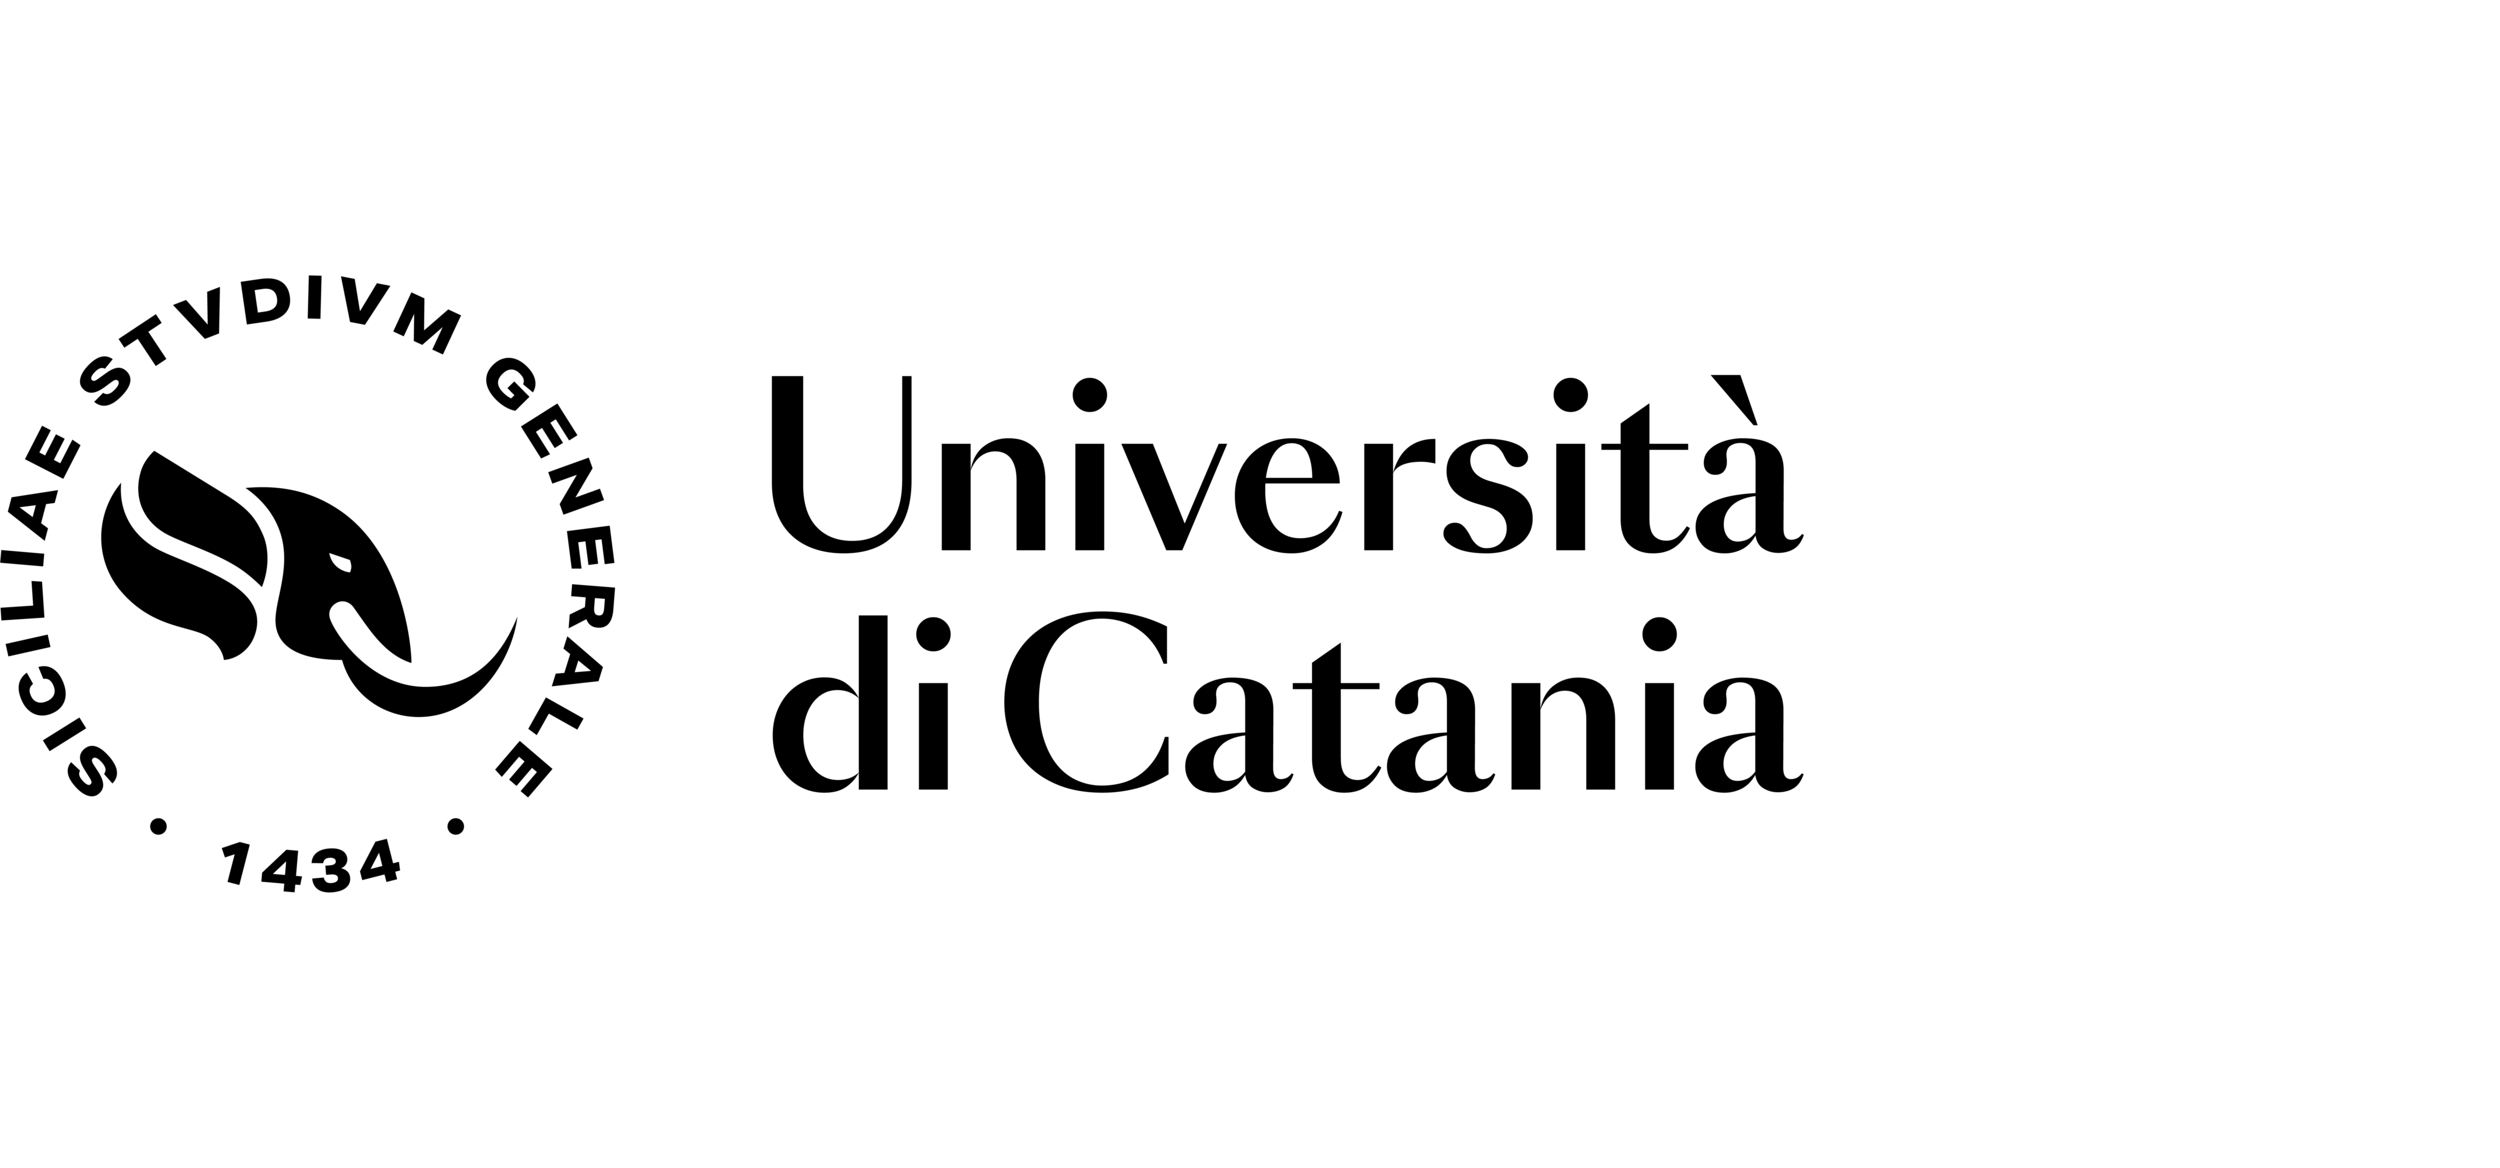
\includegraphics[width=\textwidth]{images/LogoUniCT.png}
        \end{minipage}
        \hfill
        \begin{minipage}[th!]{0.49\textwidth}
                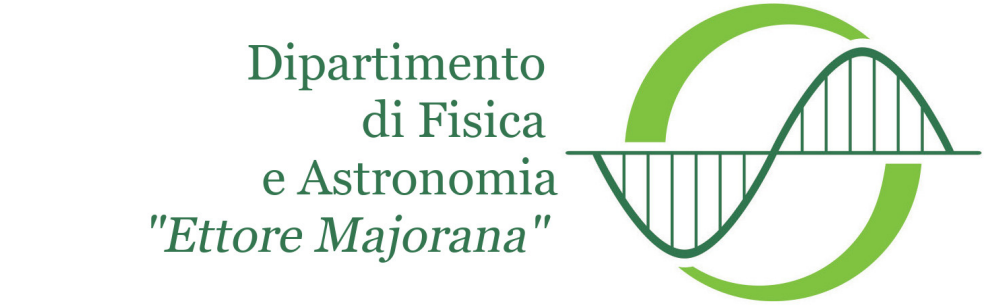
\includegraphics[width=\textwidth]{images/LogoDFA.png}
        \end{minipage}
        \large
        \textbf{CORSO DI LAUREA IN FISICA}
        \vspace{0.5cm}
        \hrule
        \vspace{3cm}
        
        \centering

        Appunti di\\\Huge{\textbf{OSCILLAZIONI E ONDE}}\\
        
        \vfill
        
        \begin{minipage}[h]{0.35\textwidth}
            \hrule
            \vspace{0.3cm}
            \small \centering
            Abstract
            \vspace{0.35cm}
            \hrule
        \end{minipage}
        
        \vfill
        
        \hrule
        \vspace{0.3cm}
        \normalsize
        \textbf{Anno Accademico 2023/2024}
    \end{center}
\end{titlepage}

\pagenumbering{Roman}
\chapter*{Prefazione}\label{s:preface}
[BOZZA] Ho deciso di stendere questa trascrizione in $\text{\LaTeX}$ degli appunti del corso Oscillazioni e Onde tenuto dal prof. Fabio Siringo durante l'A.A. 2023/2024 con l'intento di avere una raccolta organica e quanto pi\`u chiara possibile del materiale, vista l'attuale assenza di un libro di testo per il programma svolto. Nel corso della scrittura ho voluto prendermi la libert\`a di approfondire, ove lo ritenessi necessario ai fini della completezza e della chiarezza, con materiale preso da testi di Meccanica e di Matematica. \par Tengo particolarmente a sottolineare la natura personale degli appunti che non vogliono sostituirsi alle lezioni tenute dal docente o ai libri di testo, tuttavia invito chiunque lo ritenesse utile a farne un libero uso con la consapevolezza di quanto appena detto. A tal proposito, in caso il lettore dovesse riscontrare errori o volesse suggerire delle modifiche, \`e pregato di contattarmi presso:
\begin{verbatim}
    pappalardoaurelio@gmail.com
\end{verbatim}\par
Al seguente link è possibile accedere alla versione più aggiornata degli appunti: 

\begin{center}
    Ultima modifica: \today
\end{center}

% INSERIRE LINK
\chapter*{Programma del Corso}
[BOZZA] Ciao, qui andrà il programma
\begin{titlepage}
    \tableofcontents
\end{titlepage}
\pagenumbering{arabic}

%
\part{Richiami di Matematica}
\chapter{Numeri Complessi}\label{ap:A}
I numeri complessi sono la naturale estensione del campo reale $\qty(\R,+,\cdot)$ che, pur sacrificando la relazione d'ordine, permettono di avere una struttura algebricamente chiusa. \par I contenuti di questo capitolo fanno prevalentemente riferimento alle fonti \cite{Di_Fazio2013-vk,Presilla2013-uz}, con alcune modifiche e aggiunte personali.
\section{Costruzione di $\C$}
Sia $\R^2=\qty{\qty(x,y):x,y\in\R}$, poniamo $z_1=\qty(x_1,\ y_1)$, $z_2=\qty(x_2,\ y_2)$ e siano definite le operazioni:
\begin{align*}
    \func{+}{\R^2\times\R^2}{\R^2}\quad&\qty(z_1,\ z_2)\mapsto\qty(x_1+x_2,\ y_1+y_2)\\
    \func{\cdot}{\R^2\times\R^2}{\R^2}\quad&\qty(z_1,\ z_2)\mapsto\qty(x_1x_2-y_1y_2,\ x_1y_2+x_2y_1)
\end{align*}
Chiamiamo $\C=\qty(\R^2,+,\cdot)$ la struttura cos\`i costruita, che si dimostra facilmente essere un campo.
\subsection{Forme e propriet\`a dei numeri complessi}
    Definiamo \emph{modulo} di un numero complesso $z$ la quantit\`a: $$\abs{z}=\sqrt{x^2+y^2}\in\R.$$ 
    \subsubsection{Forma algebrica}
        Osserviamo che l'insieme $\qty{\qty(x,y)\in\R^2:y=0}$ \`e isomorfo a $\R$, per cui poniamo $x=\qty(x,0)$. Sia inoltre $i=\qty(0,\ 1)$, da cui:
        \begin{align*}
            &y\cdot i=\qty(y,0)\cdot(0,1)=(0,y)\\
            &i^2=\qty(0,1)\cdot\qty(0,1)=(-1,0)=-1
        \end{align*}
        Facendo la posizione $iy=\qty(0,y)$, ogni numero complesso $z=\qty(x,y)$ pu\`o essere scritto nella sua \emph{forma algebrica} $z=x+iy$, infatti: $$x+iy=\qty(x,0)+\qty(0,y)=(x,y)$$
        Dato un numero complezzo $z=x+iy$, definiamo:
        \begin{itemize}
            \item $\Re z=x$, detta \emph{parte reale} di $z$;
            \item $\Im z=iy$, detta \emph{parte immaginaria} di $z$;
            \item $\overline{z}=x-iy$, detto \emph{complesso coniugato} di $z$.
        \end{itemize}
        Vale inoltre la propriet\`a $\abs{z}=z\overline{z}$.
    \subsubsection{Forma trigonometrica ed esponenziale}
        Come noto, \`e possibile rappresentare i punti del piano $\qty(x,y)\in\R^2$, escluso $\qty(0,0)$ in coordinate polari, fissando le due coordinate $\rho$ e $\theta$, detti rispettivamente \emph{raggio} e \emph{angolo polare}. \par Pensando ai numeri complessi come punti del piano, si osserva: $$x=\rho\cos\theta,\quad y=\rho\sin\theta,$$ da cui: $$z=\rho\qty(\cos\theta+i\sin\theta),$$ che viene detta \emph{forma trigonometrica} di $z$. Segue naturalmente che:
        \begin{itemize}
            \item $\rho=\abs{z}$;
            \item $\theta$ \`e l'angolo che risolve $x=\rho\cos\theta$ e $y=\rho\sin\theta$;
            \item $\overline{z}=\rho\qty(\cos\theta-i\sin\theta)=\rho\qty[\cos\qty(-\theta)+i\sin\qty(-\theta)]$.
        \end{itemize}
        \par Consideriamo ora la quantit\`a $e^{i\theta}$ e dimostriamo che rappresenta ancora un numero complesso. \`E possibile interpretare l'esponenziale come una somma infinita di termini, esprimendo la funzione $e^z$ come serie di Taylor centrata in $0$: $$e^{i\theta}=\sum_{n=0}^{+\infty}\frac{\qty(i\theta)^n}{n!}=\sum_{n=0}^{+\infty}i^n\frac{\theta^n}{n!}=\sum_{n=0}^{+\infty}\qty(-1)^n\frac{\theta^{2n}}{\qty(2n)!}+i\sum_{n=0}^{+\infty}\qty(-1)^n\frac{\theta^{2n+1}}{\qty(2n+1)!}$$ dove \`e evidente la presenza degli sviluppi di seno e coseno, da cui: 
        \begin{equation}
            e^{i\theta}=\cos\theta+i\sin\theta,
            \label{eq:euler:1}
        \end{equation}
        la quale prende il nome di \emph{formula di Eulero}.\footnote{Da cui la pi\`u popolare \emph{identit\`a di Eulero}: $e^{i\pi}+1=0$} Segue che qualunque numero complesso $z\neq 0$ pu\`o essere espresso come: $$z=\rho\qty(\cos\theta+i\sin\theta)=\rho e^{i\theta},$$ che viene detta \emph{forma esponenziale} del numero complesso.
        \par Dalla formula di Eulero seguono altre importanti relazioni. Consideriamo ancora $z=e^{i\theta}$ e il suo coniugato, che per le precedenti \`e naturalmente $\overline{z}=e^{-i\theta}$:
        \begin{align}
            z+\overline{z}=e^{i\theta}+e^{-i\theta}=2\cos\theta\ \iff\ \cos\theta=\frac{e^{i\theta}+e^{-i\theta}}{2}\\
            z-\overline{z}=e^{i\theta}-e^{-i\theta}=2i\sin\theta\ \iff\ \sin\theta=\frac{e^{i\theta}-e^{-i\theta}}{2i}
        \end{align}
        Inoltre, per qualunque $z_1,z_2\in\C$ si ha:
            $$z_1z_2=\rho_1e^{i\theta_1}\rho_2e^{i\theta_2}=\rho_1\rho_2e^{i\qty(\theta_1+\theta_2)}.$$
        da cui:
        \begin{equation}
            \overline{z_1z_2}=\rho_1\rho_2\myexp{-i\qty(\theta_1+\theta_2)}=\rho_1\myexp{-i\theta_1}\rho_2\myexp{-i\theta_2}=\overline{z}_1\overline{z}_2
            \label{eq:prodottoconiugati}
        \end{equation}
    \section{Formula di De Moivre e radici in $\C$}
        Per poter operare al meglio coi numeri complessi, introduciamo dei metodi per eseguire con facilit\`a le operazioni di elevamento a potenza ed estrazione di radice. Consideriamo due numeri $z_1=\rho_1e^{i\theta_1}$ e $z_2=\rho_2e^{i\theta_2}$ e il loro prodotto:
            $$z_1z_2=\rho_1\rho_2e^{i\qty(\theta_1+\theta_2)}.$$
        Da questa scrittura possiamo inutire che per qualunque $z\neq 0$ e $k\in\Z$, possiamo scrivere:
        \begin{equation}
            z^k=\rho^ke^{ik\theta}=\rho^k\qty(\cos k\theta+i\sin k\theta)
            \label{eq:demoivre}
        \end{equation}
        che viene detta formula di De Moivre e pu\`o essere dimostrata per induzione su $k$.
        \par Il lettore potrebbe essere indotto a pensare che una scrittura simile sia corretta anche per gli esponenti razionali, come nel caso dell'estrazione di radice. Tuttavia \`e necessario tenere a mente che estrarre la radice $n$-esima, con $n\in\N$, di un numero complesso $a$ vuol dire risolvere l'equazione:
            $$z^n=a,$$
        che in $\C$ ha $n$ soluzioni distinte, in virt\`u del teorema fondamentale dell'algebra. Per tali soluzioni \`e ancora una volta possibile fare riferimento alla forma esponenziale e trigonometrica dei numeri complessi, infatti ricordando che per la periodicit\`a di seno e coseno $a=\rho\myexp{i\qty(\theta+2m\pi)}$, $m\in\Z$ deve essere:
            $$z^n=\rho\myexp{i\qty(\theta+2m\pi)}\ \iff\ z=\rho^{\frac{1}{n}}\myexp{i\qty(\frac{\theta+2m\pi}{n})},\quad m=0,\dots,n-1.$$ % numeri complessi
\chapter{Cenni di Analisi Complessa}\label{ap:B}
Il proposito di questo capitolo \`e quello di fornire nozioni utili al calcolo di funzioni complesse di variabile complessa dal punto di vista pi\`u pratico che teorico.
\begin{definition}[Intorno di un punto]
    
\end{definition} % analisi complessa (residui e fourier)
%
\part{Oscillazioni e Onde}
% - % - % - % - % - % - % - % - % - % - % - % - %
%  ______   ______        _____     ______      %
% /\__  _\ /\  __ \      /\  __-.  /\  __ \     %
% \/_/\ \/ \ \ \/\ \     \ \ \/\ \ \ \ \/\ \    %
%    \ \_\  \ \_____\     \ \____-  \ \_____\   %
%     \/_/   \/_____/      \/____/   \/_____/   %
% - % - % - % - % - % - % - % - % - % - % - % - %
% [ ] Sistemare introduzione (copiare il Goldstein!!! \eta^\alpha idea molto bella)
% [x] Label capitolo
% [x] Reference appendice
% [ ] Caso Anisotropo più compatto?
% [ ] Finire caso 3D!!!
% [ ] Laurearsi
% [ ] Spazio di Bruillon?
% [x] Aggiustare dimostrazione catena con q_m e N=2p+1
% [ ] Aggiustre eq del moto
% [x] Sposstare relazione di dispersione e prima parte eq moto nella sottosez precedente
% [x] Spezzare il calcolo diagon. pot. per N molle (sviluppare \zeta_n^2 a parte e poi mettere nella sommatoria)
% [ ] Condizioni iniziali eq moto N masse?
\chapter{L'Oscillatore Armonico}\label{ch:1}
\section{Introduzione}
    Dato un sistema fisico le cui configurazioni sono identificate dalle coordinate pure $q^\alpha$, dalla meccanica \`e noto che le configurazioni di equilibrio stabile si hanno in corrispondenza dei minimi del potenziale $V\qty(q^\alpha)$. Assumendo che $V$ sia una funzione almeno di classe $C^2$ e che ammetta minimo, \`e possibile effettuare una traslazione che ponga l'origine del S.d.R.\footnote{Sistema di riferimento} coincidente col punto di minimo e sviluppare in serie di Taylor/Mac Laurin il potenziale, arrestandosi al termine di secondo grado. Si ottiene dunque: $$V\qty(q^\alpha)=V\qty(\vb{0})+\pdv{V}{q^\alpha}\eval_{\vb{0}}q^\alpha+\frac{1}{2}\pdv{V}{q^\alpha}{q^\beta}\eval_{\vb{0}}q^\alpha q^\beta+R\qty(q^\alpha).$$ Ricordando che il potenziale \`e definito a meno di una costante additiva e che all'equilibrio $\displaystyle\pdv{V}{q^\alpha}\eval_{\vb{0}}=0$, e trascurando il termine infinitesimo, si pu\`o riscrivere il potenziale come:
    \begin{equation}
        V\qty(q^\alpha)=\frac{1}{2}\pdv{V}{q^\alpha}{q^\beta}\eval_{\vb{0}}q^\alpha q^\beta,
        \label{eq:potenziale:1}
    \end{equation} che non \`e altro che una forma quadratica del tipo $\displaystyle\frac{1}{2}\underline{x}^\top H_V\qty(\vb{0})\underline{x}$, con $\underline{x}\in\R^n$ un punto e $H_V\qty(\vb{0})$ la matrice Hessiana di $V$ calcolata in $\vb{0}$.
    \par Ovviamente questo \`e soltanto un modello approssimato che pu\`o essere applicato in un intorno del minimo. Se ci si allontana troppo, le discordanze tra il modello e le misure che si riscontrano prendono il nome di \emph{effetti anarmonici}.
\section{Oscillatore armonico unidimensionale}
    Applichiamo quanto detto al caso unidimensionale. Siano $A\subseteq\R$ un aperto, $\func{V}{A}{\R}$ una funzione di classe $C^2$ e $x_0\in A$ un punto di minimo per $V$. La \eqref{eq:potenziale:1} diventa:
        $$V(x-x_0)=\frac{1}{2}\dv[2]{V}{x}\eval_{x_0}\qty(x-x_0)^2;$$
    ponendo $u=x-x_0$, si effettua la traslazione che pone il punto di minimo nell'origine, per cui si ottiene:
        $$V(u)=\frac{1}{2}\dv[2]{V}{x}\eval_{0}u^2.$$
    \par A questo punto risulta evidente la somiglianza con il potenziale della forza elastica. Ponendo $\displaystyle k=\dv[2]{V}{x}\eval_{x_0}$ e prendendone il "gradiente" (derivata prima) cambiato di segno, si ottiene l'espressione della forza elastica tramite la legge di Hooke:
        $$V\qty(u)=\frac{1}{2}ku^2\ \implies\ \vb{F\qty(\vb{u})}=-\dv{V}{x}\vu{i}=-k\vb{u},$$
    da cui l'equazione del moto: $m\ddot{u}=-ku$, che \`e lineare omogenea del secondo ordine.
    \par Ponendo $\frac{k}{m}=\omega^2$, si pu\`o scrivere $\ddot{u}=-\omega^2u$, di cui due soluzioni linearmente indipendenti sono $\cos\qty(\omega t)$ e $\sin\qty(\omega t)$. L'integrale generale \`e quindi $$u\qty(t)=c_1\cos\qty(\omega t)+c_2\sin\qty(\omega t)$$ con $c_1,c_2\in\R$, o alternativamente, ponendo $c_1=A\cos\phi$ e $c_2=-A\sin\phi$, ancora con $A,\phi\in\R$,
        $$u\qty(t)=A\cos\qty(\omega t+\phi).$$
    In tal caso, $A$ si dice \emph{ampiezza}, $\omega$ si dice \emph{pulsazione} o \emph{frequenza angolare} e $\omega t+\phi$ si dice \emph{fase}.
\section{Oscillatore armonico bidimensionale}
    Proviamo ora passo passo ad aumentare il numero di dimensioni, per semplicit\`a iniziamo da 2. Quando vi \`e pi\`u di un grado di libert\`a, \`e importante distinguere i casi in base alle simmetrie che il sistema presenta. Se il potenziale \`e invariante per rotazioni, diciamo che l'oscillatore armonico \`e \emph{isotropo}, altrimenti lo diciamo \emph{anisotropo}.
    \subsection{Oscillatore isotropo}
        Come prima, supponiamo di avere $\func{V}{A\subseteq{\R^2}}{\R}$, definito dalla legge:
            $$V\qty(x,y)=\frac{1}{2}m\omega^2\qty(x^2+y^2),$$
        ove si \`e usata la relazione $k=m\omega^2$. Notiamo subito che il potenziale \`e invariante per rotazioni in quanto le curve equipotenziali sono circonferenze centrate nell'origine\footnote{Immaginiamo di trovarci gi\`a nel sistema di riferimento scelto in modo da collocare un punto di minimo di $V$ nell'origine, se cos\`i non fossoe, \`e sempre possibile ricondursi a quel caso con una traslazione}. Di conseguenza $V$ si spezza facilmente in:
            $$V\qty(x,y)=\frac{1}{2}m\omega^2x^2+\frac{1}{2}m\omega^2y^2$$
        e derivando si ottengono quindi le due equazioni del moto gi\`a disaccoppiate.
        \begin{equation*}
        \begin{cases}
            \ddot{x}=-\omega^2x\\
            \ddot{y}=-\omega^2y
        \end{cases}
        \end{equation*}
        le cui soluzioni sono nuovamente le funzioni $x\qty(t)=A_1\cos(\omega t+\phi_1)$ e $y\qty(t)=A_2\cos(\omega t+\phi_2)$, definite a meno di quattro costanti arbitrarie. Fissando le condizioni iniziali: $x\qty(0)$, $\dot{x}\qty(0)$, $y\qty(0)$ e $\dot{y}\qty(0)$, \`e possibile trovare l'unica soluzione del problema di Cauchy.
    \subsection{Oscillatore anisotropo}
        Affrontiamo adesso il caso di un potenziale che non presenti simmetrie per rotazione, ad esempio:
            $$V\qty(x,y)=\frac{1}{2}m\omega^2x^2+\frac{1}{2}m\omega^2y^2+2\gamma xy,\quad\gamma>0.$$
        \subsubsection{Diagonalizzazione del potenziale}
            Come \`e noto dalla \eqref{eq:potenziale:1}, \`e possibile riscrivere il potenziale come forma quadratica:
                $$\frac{1}{2}m\omega^2\mqty(x&y)\mqty[1 & \frac{\gamma}{m\omega^2} \\ \frac{\gamma}{m\omega^2} & 1]\mqty(x\\y).$$
            Poich\`e la matrice dei coefficienti \`e simmetrica, per il teorema spettrale \`e diagonalizzabile ed esiste quindi un cambio di coordinate che pone la forma quadratica in forma canonica, disaccoppiando di conseguenza le equazioni del moto.
            \par Le nuove coordinate sono quelle identificate da una base (ortonormale) di autovettori della matrice, cerchiamo quindi gli zeri del polinomio caratteristico:
                $$P\qty(\lambda)=\det\mqty[1-\lambda & \frac{\gamma}{m\omega^2} \\ \frac{\gamma}{m\omega^2} & 1-\lambda]=\qty(1-\lambda)^2-\frac{\gamma^2}{m^2\omega^4}=0\ \implies\ \lambda_{\pm}=1\pm\frac{\gamma}{m\omega^2}.$$
            Calcoliamo ora gli autovettori\footnote{O meglio, le loro componenti rispetto alla base canonica di $\R^2$: $\qty{e_1,e_2}$} $Q_{\pm}$ associati agli autovalori $\lambda_{\pm}$, risolvendo i due sistemi:
            \begin{equation*}
            \begin{cases}
                \displaystyle\qty(1-\lambda_{\pm})x+\frac{\gamma}{m\omega^2}y=0\\\\
                \displaystyle\qty(1-\lambda_{\pm})y+\frac{\gamma}{m\omega^2}x=0
            \end{cases}
            \end{equation*}
            e ottenendo quindi le componenti degli autovettori, $\qty[Q_{\pm}]=[x,\pm x]$. Scegliamo quindi due autovettori normalizzati:
                $$Q_{+}=\frac{1}{\sqrt{2}}\mqty(1 \\ -1),\quad Q_{-}=\frac{1}{\sqrt{2}}\mqty(1 \\ 1)$$
            e la conseguente matrice di rotazione:
                $$P=\frac{1}{\sqrt{2}}\mqty[1 & 1 \\ -1 & 1]\quad\text{tale che}\quad\mqty[1-\frac{\gamma}{m\omega^2} & 0 \\ 0 & 1+\frac{\gamma}{m\omega^2}]=P^\top\mqty[1 & \frac{\gamma}{m\omega^2} \\ \frac{\gamma}{m\omega^2} & 1]P.$$
            Troviamo ora $e_1$ ed $e_2$ nelle nuove coordinate tramite i due sistemi vettoriali:
            \begin{align*}
                e_1=xQ_++yQ_-\ & \iff\ \mqty(1 \\ 0)=\frac{1}{\sqrt{2}}\qty[x\mqty(1 \\ -1)+y\mqty(1 \\ 1)] \\\\
                e_2=xQ_++yQ_-\ & \iff\ \mqty(0 \\ 1)=\frac{1}{\sqrt{2}}\qty[x\mqty(1 \\ -1)+y\mqty(1 \\ 1)] 
            \end{align*}
            da cui $e_1=\frac{1}{\sqrt{2}}\qty(Q_++Q_-)$, $e_2=\frac{1}{\sqrt{2}}\qty(Q_+-Q_-)$. Trasformando le coordinate si ottiene il nuovo potenziale:
                $$V\qty(Q_+,Q_-)=\frac{1}{2}m\omega^2\qty(Q_+^2+Q_-^2)+\frac{\gamma}{2}\qty(Q_+^2-Q_-^2),$$
            che si spezza facilmente in:
                $$V\qty(Q_+,Q_-)=\frac{1}{2}m\Omega_+^2Q_+^2+\frac{1}{2}m\Omega_-^2Q_-^2,$$
            avendo fatto la posizione $\Omega_\pm^2=\omega^2\qty(1\pm\frac{\gamma}{m\omega^2})$.
        \subsubsection{Equazioni del moto}
            A questo punto trovare e risolvere le equazioni del moto \`e banale:
                $$\ddot{Q}_\pm=-\Omega_\pm^2Q_\pm\ \implies\ Q_\pm\qty(t)=A_\pm\cos\qty(\Omega_\pm t+\phi_\pm),$$
            e attraverso la trasformazione inversa \`e possibile ricavare le $x\qty(t)$, $y\qty(t)$:
            \begin{align*}
                & x\qty(t)=\frac{Q_+\qty(t)+Q_-\qty(t)}{\sqrt{2}}=\frac{1}{\sqrt{2}}\qty[A_+\cos\qty(\Omega_+t+\phi_+)+A_-\cos\qty(\Omega_-t+\phi_-)] \\
                & y\qty(t)=\frac{Q_+\qty(t)-Q_-\qty(t)}{\sqrt{2}}=\frac{1}{\sqrt{2}}\qty[A_+\cos\qty(\Omega_+t+\phi_+)-A_-\cos\qty(\Omega_-t+\phi_-)]
            \end{align*}
            Dove, come ci aspettavamo, $A_\pm$ e $\phi_\pm$ sono quattro costanti reali determinabili conoscendo le condizioni iniziali.
        \subsubsection{Energia cinetica}
            Avendo operato una rotazione che non altera la metrica, ci aspettiamo che l'energia cinetica $T$ resti invariata da un S.d.R. all'altro.
            \par Dalla definizione $\displaystyle T=\frac{1}{2}m\norm{\vb{v}}^2$, sviluppando il prodotto scalare otteniamo: $$T=\frac{1}{2}m\qty(\dot{x}^2+\dot{y}^2)$$ Derivando le equazioni di trasformazione invece troviamo:
            \begin{align*}
                &\dv{x}{t}=\dv{t}\frac{Q_++Q_-}{\sqrt{2}}=\frac{\dot{Q}_++\dot{Q}_-}{\sqrt{2}}\\
                &\dv{y}{t}=\dv{t}\frac{Q_+-Q_-}{\sqrt{2}}=\frac{\dot{Q}_+-\dot{Q}_-}{\sqrt{2}}
            \end{align*}
            e sostituendo nell'energia cinetica:
                $$T=\frac{1}{2}m\qty[\frac{\qty(\dot{Q}_++\dot{Q}_-)^2}{2}+\frac{\qty(\dot{Q}_++\dot{Q}_-)^2}{2}]=\frac{1}{2}m\qty(\dot{Q}_+^2+\dot{Q}_-^2),$$
            che prova quanto affermato.
\section{Oscillatore a tre gradi di libert\`a}
    Proviamo ora a generalizzare ulteriormente quanto detto fin'ora per sistemi che abbiano pi\`u di due gradi di libert\`a. Iniziamo considerando il caso di tre masse legate da molle ideali con estremi liberi, per poi affrontare il caso con condizioni armoniche al contorno e successivamente generalizzare a $n$ masse.
    \subsection{Tre masse a estremi liberi}
        Prendiamo in esame un sistema fisico formato da tre masse uguali $m$ vincolate a muoversi sull'asse $x$, collegate da due molle di costante $k=m\omega^2$.
        \par Le configurazioni di questo sistema fisico sono identificate dalle coordinate generalizzate $q^\alpha=\qty{x,y,z}$ che indicano la posizione delle tre massse rispetto all'origine. Sul sistema agiscono due forze, entrambe forze elastiche, che dipendono dalle due distanze $\qty(y-x)$ e $\qty(z-y)$. Possiamo facilmente calcolare il potenziale elastico delle molle:
            $$V\qty(x,y,z)=\frac{1}{2}m\omega^2\qty(x-y)^2+\frac{1}{2}m\omega^2\qty(y-z)^2=$$
            $$=\frac{1}{2}m\omega^2\qty(x^2-2xy+2y^2-2yz+z^2),$$
        la cui matrice associata \`e $\displaystyle B=\mqty[1 & -1 & 0 \\ -1 & 2 & -1 \\ 0 & -1 & 1]$. Procediamo come precedentemente per diagonalizzare il potenziale:
            $$P\qty(\lambda)=\det\mqty[1-\lambda & -1 & 0 \\ -1 & 2-\lambda & -1 \\ 0 & -1 & 1-\lambda]=\lambda\qty(1-\lambda)\qty(\lambda-3).$$
        Gli autovalori sono $\lambda_0=0$, $\lambda_1=1$ e $\lambda_3=3$. Dal calcolo degli autovettori associati otteniamo le componenti dei vettori normalizzati:
            $$q_0=\frac{1}{\sqrt{3}}\mqty(1 \\ 1 \\ 1),\quad q_1=\frac{1}{\sqrt{2}}\mqty(1 \\ 0 \\ -1),\quad q_3=\frac{1}{\sqrt{6}}\mqty(1 \\ -2 \\ 1),$$
        con cui possiamo costruire la matrice di rotazione $P$ tale che $\det P=1$ contenente $q_3$, $q_1$ e $q_0$ sulle colonne, che diagonalizza il potenziale:
            $$D=P^\top BP\ \iff\ PDP^\top=B.$$
        Sostituendo $B$ nella forma quadratica:
            $$V\qty(x,y,z)=\frac{1}{2}m\omega^2\mqty(x & y & z)PBP^\top\mqty(x\\y\\z),$$
        dove, come prima \`e stato mostrato in maniera pi\`u esplicita, $P^\top\mqty(x\\y\\z)$ trasforma le coordinate, il potenziale assume la forma:
            $$V(q_3,q_1,q_0)=\frac{1}{2}m\omega^2\mqty(q_3 & q_1 & q_0)\mqty[\dmat[0]{3,1,0}]\mqty(q_3 \\ q_1 \\ q_0)=\frac{1}{2}m\omega^2\qty(3q_3^2+q_1^2)$$
        e, ponendo di nuovo $\Omega_3^2=3\omega^2$ e $\Omega_1^2=\omega^2$, otteniamo le equazioni del moto:
        \begin{equation*}
        \begin{cases}
            \ddot{q}_0=0\\
            \ddot{q}_1=-\Omega_1^2q_1\\
            \ddot{q}_3=-\Omega_3^2q_3
        \end{cases}
        \iff\
        \begin{cases}
            q_0\qty(t)=v_0t+s_0\\
            q_1\qty(t)=A_1\cos\qty(\Omega_1 t+\phi_1)\\
            q_3\qty(t)=A_3\cos\qty(\Omega_3 t+\phi_3)
        \end{cases}
        \end{equation*}
        Applicando la trasformazione di coordinate inversa data da $\mqty(x \\ y \\ z)=P\mqty(q_3 \\ q_1 \\ q_0)$ possiamo trovare $x\qty(t)$, $y\qty(t)$ e $z\qty(t)$:
        \begin{align*}
            &x\qty(t)=\frac{1}{\sqrt{3}}\qty(v_0t+s_0)+\frac{A_1}{\sqrt{2}}\cos\qty(\Omega_1t+\phi_1)+\frac{A_3}{\sqrt{6}}\cos\qty(\Omega_3t+\phi_3)\\
            &y\qty(t)=\frac{1}{\sqrt{3}}\qty(v_0t+s_0)-\frac{2A_3}{\sqrt{6}}\cos\qty(\Omega_3t+\phi_3)\\
            &z\qty(t)=\frac{1}{\sqrt{3}}\qty(v_0t+s_0)-\frac{A_1}{\sqrt{2}}\cos\qty(\Omega_1t+\phi_1)+\frac{A_3}{\sqrt{3}}\cos\qty(\Omega_3t+\phi_3)
        \end{align*}
        Come ci potevamo aspettare dalla presenza di tre equazioni lineari del secondo ordine, le equazioni del moto sono definite a meno di sei costanti arbitrarie: $v_0$, $s_0$, $A_1$, $\phi_1$, $A_3$ e $\phi_3$. \`E inoltre importante sottolineare il significato fisico legato alla presenza di $\lambda_0=0$ tra gli autovalori: possiamo notare che l'equazione del moto associata alla coordinata $q_0$ costituisce un moto rettilineo uniforme, e non oscillatorio, che suggerisce una simmetria del sistema per traslazioni.
        \par A questo punto risulta utile introdurre il concetto di \emph{modi normali di oscillazione}.
    \subsection{Tre masse con condizioni periodiche al contorno}
        Supponiamo adesso di avere tre masse disposte come nell'esempio precedente ma con l'ulteriore condizione che la prima e la terza massa interagiscano per mezzo di una terza molla di caratteristiche uguali alle altre due. Questa situazione fisica pu\`o essere meglio visualizzata come se sia le masse che le molle fossero vincolate a scorrere su di una circonferenza rigida $\gamma$ priva di attrito.
        \par Anche in questo caso possiamo ricorrere alle coordinate pure $x$, $y$ e $z$ che stavolta rappresentano le ascisse curvilinee condotte da un arbitraio punto $O\in\gamma$ fino a individuare la posizione delle tre masse. Il potenziale, similmente a prima, si presenta come: 
        \begin{multline*}
            V=\frac{1}{2}\omega^2\qty[\qty(x-y)^2+\qty(y-z)^2+\qty(z-x)^2]=\\=\frac{1}{2}m\omega^2\mqty(x & y & z)\mqty[\dmat[-1]{2,2,2}]\mqty(x \\ y \\ z)=\frac{1}{2}m\omega^2\underline{x}^\top B\underline{x}.
        \end{multline*}
        Eseguiamo il solito procedimento per diagonalizzare $B$:
            $$P\qty(\lambda)=\det\mqty[\dmat[-1]{2-\lambda,2-\lambda,2-\lambda}]=-\lambda\qty(\lambda-3)^2=0,$$
        che d\`a gli autovalori $\lambda_0=0$ e $\lambda_3=3$ doppio. Gli autovettori normalizzati che se ne ricavano sono:
            $$q_0=\frac{1}{\sqrt{3}}\mqty(1 & 1 & 1)\quad q_{3,1}=\frac{1}{\sqrt{}}\mqty( & & )$$
\section{Oscillatore a $N$ gradi di libert\`a}\label{s:Ngradi}
    Generalizziamo definitivamente il problema considerando il caso di una catena di $N$ masse $\mu$ collegate a due a due da molle di costante elastica $k=\mu\omega^2$ con condizioni periodiche al contorno.
    \par Supponiamo per comodit\`a $N$ dispari, denotiamo con $a$ il passo reticolare, con $x_n=na$ la posizione di equilibrio dell'$n$-esima massa $\qty(n=0,\dots,N-1)$, con $L=Na$ la lunghezza della catena e con $M=N\mu$ la massa totale. Sia inoltre la funzioni $\zeta_n$ la dislocazione dell'$n$-esima massa dalla posizione di equilibrio $x_n$. Richiedere che le condizioni al contorno siano periodiche vuol dire supporre che l'ultima massa possa interagire con la prima, come se la catena formasse un cerchio. In termini matematici questo si traduce in:
    \begin{align}
        &x_{n+N}=x_n+L\equiv x_n \label{eq:period:1}\\
        &\zeta_{n+N}\equiv \zeta_n \label{eq:period:2}
    \end{align}
    Il potenziale di un tale sistema ha forma:
    \begin{equation}
        V=\frac{1}{2}\mu\omega^2\sum_n\qty(\zeta_{n+1}-\zeta_n)^2.
        \label{eq:potenziale:2}
    \end{equation}
    \subsection{Ricerca dei modi normali di oscillazione}
        A questo punto desideriamo provare che le seguenti relazioni costituiscono il cambio di coordinate che permette di passare dalle $\zeta_n$ alle $Q_q$ ove il potenziale \`e diagonalizzato:
        \begin{align}
            &\zeta_n=\frac{1}{\sqrt{N}}\sum_m\myexp{iq_mx_n}Q_{q_m} \label{eq:cambio:1}\\
            &Q_{q_m}=\frac{1}{\sqrt{N}}\sum_n \myexp{-iq_mx_n}\zeta_n \label{eq:cambio:2}
        \end{align}
        Allo scopo di dileguare eventuali perplessit\`a, vorrei giustificare rapidamente la presenza di esponenziali complessi nelle relazioni appena enunciate. Ci si potrebbe aspettare infatti, che le trasformazioni da cercare siano simili a quelle viste nei casi semplificati a due e tre dimensioni: somme di funzioni trigonometriche con opportuni coefficienti. Volendo, potremmo affrontare questo problema proprio in questo modo, se non fosse che ci\`o renderebbe i calcoli ben pi\`u tediosi, quando invece operare con gli esponenziali complessi elimina questo problema. Infatti, basta tenere a mente che $\myexp{i\theta}=\cos\theta+i\sin\theta$ e che di consguenza ci baster\`a prendere la parte reale della soluzione per raggiungere il nostro obiettivo. Sostanzialmente stiamo affrontando un problema di moto armonico in $\R$ risolvendo il corrispettivo problema di `moto circolare' in $\C$ e `proiettandolo' su $\R$. Si rimanda all'Appendice \ref{ap:A} per qualche cenno in pi\`u ai numeri complessi.
        \par Osserviamo subito che da \eqref{eq:period:1} e \eqref{eq:cambio:1} \`e possibile conoscere l'intervallo in cui variano le $q_m$:
            $$\myexp{iqx_{n+N}}=\myexp{iqx_n}\ \iff\ \myexp{iq_mna}\myexp{iq_mL}=\myexp{iq_mna}\ \iff\ \myexp{iq_mL}=1,$$
        per cui deve essere $q_mL=2m\pi$, con $m\in\Z$. Sostituendo $L$ otteniamo:
        \begin{equation}
            q_m=\frac{2m\pi}{L}=\frac{2\pi}{a}\frac{m}{N}
            \label{eq:q}
        \end{equation}
        Dal momento che i gradi di libert\`a sono $N$, prevediamo che siano presenti proprio $N$ modi normali al variare di $q_m$, per cui possiamo scegliere $N$ diversi valori di $q_m$ al variare di $m\in\Z$. Risulta opportuna la scelta di un intervallo simmetrico $\displaystyle m\in\left[-\frac{N-1}{2};\frac{N-1}{2}\right]$, in modo che si abbia $\displaystyle q_m\in\left[-\frac{\pi}{a};\frac{\pi}{a}\right]$. Per compattezza della notazione, questo fatto sar\`a omesso nella scrittura degli indici della sommatoria laddove ci\`o non possa causare ambiguit\`a. 
        \par Prima di proseguire oltre con la risoluzione del problema, anteponiamo dei risultati utili:
        \begin{lemma} \label{lm:delta}
            Sotto le ipotesi del problema valgono le seguenti relazioni:
            \begin{align}
                &\sum_{n}\myexp{iq_mx_n}=N\delta_{q_m,0} &n=0,\dots,N-1 \label{eq:delta:1}\\
                &\sum_{m}\myexp{-iq_mx_n}=N\delta_{n,0} &m\in\left[-\frac{N-1}{2};\frac{N-1}{2}\right] \label{eq:delta:2}
            \end{align}
        ove $\delta_{\alpha,\beta}$ \`e la Delta di Kronecker.
        \end{lemma}
        \begin{proof}
            Proviamo la \eqref{eq:delta:1}.
            \par Se $q_m=0$, banalmente:
                $$\sum_{n=0}^{N-1}1=N.$$
            \par Se $q_m\neq0$, osserviamo che si pu\`o scrivere:
                $$\sum_{n=0}^{N-1} \myexp{iq_mx_n}=\sum_{n=0}^{N-1} \myexp{iq_mna}=\sum_{n=0}^{N-1}\qty(\myexp{iq_ma})^n=\frac{1-\myexp{iq_mNa}}{1-\myexp{iq_ma}}$$
            essendo il termine generale della successione delle somme parziali di una serie geometrica di ragione $\myexp{iq_ma}$. Sostituendo la \eqref{eq:q} si vede subito che tale somma risulta $0$. \\ Allo stesso modo si prova la \eqref{eq:delta:2}.
        \end{proof}
        \subsubsection{Invertibilit\`a}
            Verifichiamo adesso che le trasformazioni \eqref{eq:cambio:1} e \eqref{eq:cambio:2} sono l'una l'inversa dell'altra mostrando che la loro composizione restituisce l'identit\`a:
                $$\zeta_n=\frac{1}{\sqrt{N}}\sum_{m}\myexp{iq_mx_n}\qty(\frac{1}{\sqrt{N}}\sum_{p=0}^{N-1}\myexp{-iq_mx_p}\zeta_p)=\frac{1}{N}\sum_{p,m}\myexp{iq_m\qty(x_n-x_p)}\zeta_p.$$
            Poich\'e $\zeta_p$ non dipende da $q$, \`e possibile estrarlo dalla rispettiva sommatoria:
                $$\zeta_n=\frac{1}{N}\sum_p\zeta_p\qty[\sum_m \myexp{iq_m\qty(x_n-x_p)}]$$
            dove per il Lemma \ref{lm:delta} si pu\`o scrivere:
                $$\zeta_n=\frac{1}{N}\sum_p\zeta_p\delta_{n,p}=\zeta_n$$
            che \`e appunto l'identit\`a.
        \subsubsection{Diagonalizzazione del potenziale}
            Ci chiediamo adesso se questo cambio di coordinate ci fornisca i modi normali di oscillazione del sistema, diagonalizzando il potenziale \eqref{eq:potenziale:2}. Studiamo la seguente quantit\`a:
            \begin{multline*}
                \zeta_n^2=\frac{1}{N}\qty(\sum_m\myexp{iq_mx_n}Q_{q_m})^2=\frac{1}{N}\qty(\sum_m\myexp{iq_mx_n}Q_{q_m})\Biggl(\sum_{m} \myexp{iq_{m'}x_n}Q_{q_{m'}}\Biggr)=\\=\frac{1}{N}\sum_{m,m'}Q_{q_m}Q_{q_{m'}}\myexp{i\qty(q_m+q_{m'})x_n},
            \end{multline*}
            sommiamo quindi su $n$ e applichiamo ancora il Lemma \ref{lm:delta} dopo aver raccolto i termini comuni:
            \begin{multline*}
                \sum_n\zeta_n^2=\frac{1}{N}\sum_{m,m'}Q_{q_m}Q_{q_{m'}}\sum_n\myexp{i\qty(q_m+q_{m'})x_n}=\\=\frac{1}{N}\sum_{m,m'}Q_{q_m}Q_{q_{m'}}N\delta_{q_m,-q_{m'}}=\sum_mQ_{q_m}Q_{-q_{m'}}.
            \end{multline*}
            \par Prima di proseguire ulteriormente, facciamo delle considerazioni utili. Ricordiamo che le $\zeta_n$ sono funzioni reali e quindi deve essere $\zeta_n^*=\zeta_n$.\footnote{Con $\zeta_n^*$ indichiamo il complesso coniugato di $\zeta_n$} Inoltre, dalla \eqref{eq:cambio:1}, possiamo ricavare $\zeta_n^*$ tenendo a mente che l'indice $m$ \`e saturato dalla sommatoria e quindi nulla vieta di `cambiargli il nome' in $-m$. Inoltre, per la definizione di $q_m$ \eqref{eq:q} si evince che $q_{-m}=-q_m$. Per cui:
                $$\zeta_n^*=\frac{1}{\sqrt{N}}\sum_m\myexp{-iq_mx_n}Q_{q_m}^*=\frac{1}{\sqrt{N}}\sum_{-m}\myexp{iq_mx_n}Q_{-q_{m}}^*,$$
            dove, nello scrivere la seconda uguaglianza, \`e stato sfruttato il fatto che l'indice $m$ e che dalla Segue naturalmente:
            \begin{equation}
                \zeta_n=\zeta_n^*\ \iff\ Q_{q_m}=Q_{-{q_m}}^*\ \iff\ Q_{-{q_m}}=Q_{q_m}^*.
                \label{eq:QQ}
            \end{equation}
            \mycomment{
                        Supponendo $Q=\alpha\qty(q)+i\beta\qty(q)$ e sostituendo quanto trovato nei conti precedenti si ottiene:
                        \begin{equation}
                            \sum_n\zeta_n^2=\sum_qQ_qQ_q^*=\sum_q\qty[\alpha^2\qty(q)+\beta^2\qty(q)]
                            \label{eq:sommazetaquadro}
                        \end{equation}
            }
            \par A questo punto possiamo scrivere per esteso il potenziale, richiamando la \eqref{eq:potenziale:2}:
                $$V=\frac{1}{2}\mu\omega^2\sum_n\qty(\zeta_{n+1}-\zeta_n)^2$$
            Valutiamo la quantit\`a tra parentesi:
                $$\zeta_{n+1}-\zeta_n=\frac{1}{\sqrt{N}}\sum_mQ_{q_m}\qty(\myexp{iq_mx_{n+1}}-\myexp{iq_mx_n})=\frac{1}{\sqrt{N}}\sum_mQ_{q_m}\myexp{iq_mx_n}\qty(\myexp{iq_ma}-1)$$
            e inseriamola nel potenziale $V$ che, una volta sviluppato il quadrato similmente a prima e applicata la \eqref{eq:QQ}, diventa:
            \begin{multline*}
                V=\frac{1}{2}\frac{\mu\omega^2}{N}\sum_n\sum_{m,m'}\myexp{iq_mx_n}\qty(\myexp{iq_ma}-1)\myexp{iq_{m'}x_n}\bigl(\myexp{iq_{m'}a}-1\bigr)Q_{q_m}Q_{q_{m'}}=\\=\frac{1}{2}\mu\omega^2\sum_{m,m'}\delta_{m,-q_{m'}}\qty(\myexp{iq_ma}-1)\bigl(\myexp{iq_{m'}}-1\bigr)Q_{q_m}Q_{q_{m'}}=\\=\frac{1}{2}\mu\omega^2\sum_m\qty(\myexp{iq_ma}-1)\qty(\myexp{-iq_ma}-1)Q_{q_m}Q_{-q_m}=\\=\frac{1}{2}\mu\omega^2\sum_m\qty(\myexp{iqa}-1)\qty(\myexp{-iq_ma}-1)Q_{q_m}Q_{q_m}^*
            \end{multline*}
            Da cui la nuova espressione di $V$:
            \begin{equation}
                V=\frac{1}{2}\mu\omega^2\sum_m\qty(\myexp{iq_ma}-1)\qty(\myexp{-iq_ma}-1)\norm{Q_{q_m}}^2
            \end{equation}
            che non \`e altro che una forma quadratica nelle variabili $Q_{q_m}$ la cui matrice dei coefficienti \`e diagonale e contiene gli autovalori $\qty(\myexp{iq_ma}-1)\qty(\myexp{-iq_ma}-1)$, ciascuno associato all'autovettore $Q_{q_m}$ corrispondente. Chiamiamo i vettori di base di queste nuove coordinate $Q_{q_m}$, \emph{modi normali di oscillazione} del sistema. Queste coordinate in cui il potenziale \`e diagonale costuituiscono diversi `modi' di oscillare del sistema fisico, ciascuno linearmente indipendente dagli altri. Di conseguenza qualunque moto periodico del sistema pu\`o essere espresso come combinazione lineare dei modi normali.
            \par Possiamo maneggiare ulteriormente la forma del potenziale moltiplicando e dividendo il risultato ottenuto per $\displaystyle 4i^2\myexp{i\frac{q_ma}{2}}$:
                $$V=\frac{-4}{2}\mu\omega^2\sum_m\frac{\myexp{i\frac{q_ma}{2}}-\myexp{-i\frac{q_ma}{2}}}{2i}\frac{\myexp{-i\frac{q_ma}{2}}-\myexp{i\frac{q_ma}{2}}}{2i}Q_{q_m}^2,$$
            dove riconosciamo le formule di Eulero per il seno:
                $$V=2\mu\omega^2\sum_m\sin^2\qty(\frac{q_ma}{2})Q_{q_m}^2.$$
            Notiamo infine che ponendo:
            \begin{equation}
                \Omega_{q_m}=2\omega\sin\qty(\frac{q_ma}{2}),
                \label{eq:dispersione:1}
            \end{equation}
            il potenziale assume la forma pi\`u compatta ed elegante:
            \begin{equation}
                V=\frac{1}{2}\mu\sum_m\Omega_{q_m}^2Q_{q_m}^2.
                \label{eq:potenziale:3}
            \end{equation}
        \subsubsection{Relazione di dispersione}
            \`E opportuno soffermarsi un istante a osservare la posizione \eqref{eq:dispersione:1}. Essa prende il nome di \emph{relazione di dispersione} e ci permette di esprimere la frequenza di oscillazione di ciacun modo normale in funzione del vettore d'onda $q_m$ associato. In questo caso notiamo che la relazione non \`e lineare, ma pu\`o essere approssimata come tale per i $q_m$ prossimi allo $0$ o se il passo $a$ \`e sufficientemente piccolo da rendere infinitesimo l'argomento del seno. Qualora ci\`o fosse possibile, la relazione di dispersione assumerebbe la forma $\Omega_{q_m}=\omega aq_m$, dove la quantit\`a $\omega a$ ha le dimensioni di una velocit\`a.
            \par L'argomento sar\`a ripreso pi\`u approfonditamente nel paragrafo \ref{s:casocontinuo} sullo studio del limite per $a\to 0$.
    \subsection{Energia cinetica e Lagrangiana}
        Applichiamo al sistema la definizione di energia cinetica che, essendo invariante per rototraslazioni, deve risultare uguale sia nelle $\dot{\zeta}_n$ che nelle $\dot{Q}_{q_m}$. Consideriamo:
            $$\dot{\zeta}_n=\frac{1}{\sqrt{N}}\sum_m\myexp{iq_mx_n}\dot{Q}_{q_m}.$$
        Con passaggi del tutto analoghi ai precedenti, troviamo:
            $$T=\frac{1}{2}\mu\sum_n\dot{\zeta}_n^2=\frac{1}{2}\mu\sum_m\dot{Q}_{q_m}\dot{Q}^*_{q_m}=\frac{1}{2}\mu\sum_m\dot{Q}_{q_m}^2$$
        La Lagrangiana risulta quindi:
        \begin{equation}
            \LL=T-V=\frac{1}{2}\mu\sum_m\qty(\dot{Q}_{q_m}^2-\Omega_{q_m}^2Q_{q_m}^2).
            \label{eq:mollelagrangiana}
        \end{equation}
    \subsection{Risoluzione delle equazioni del moto}
        Scriviamo ora le $N$ equazioni del moto sostituendo la \eqref{eq:mollelagrangiana} nelle equazioni di Eulero-Lagrange:
            \begin{equation}
                \lagrange{\LL}{Q_{q_m}}{\dot{Q}_{q_m}}=0\ \implies\ \ddot{Q}_{q_m}=-\Omega_{q_m}^2Q_{q_m},
                \label{eq:eqmoto:1}
            \end{equation}
        le cui soluzioni sono del tipo $\displaystyle Q_{q_m}\qty(t)=\myexp{\pm i\Omega_{q_m}t}$.
        \subsubsection{Integrale generale}
            Le generiche soluzioni di \eqref{eq:eqmoto:1} dipenderanno da due costati arbitrarie $A_{q_m}^\pm\in\C$ determinate dalle condizioni iniziali e avranno forma:
                $$Q_{q_m}\qty(t)=A_{q_m}^+\myexp{i\Omega_{q_m}t}+A_{q_m}^-\myexp{-i\Omega_{q_m}t}.$$
            Dal momento che le $A_{q_m}^\pm$ sono complesse, possiamo esprimerle in forma esponenziale come $A_{q_m}^\pm=\rho_{q_m}^\pm \myexp{i\phi_{q_m}^\pm}$, da cui:
                $$Q_{q_m}\qty(t)=\rho_{q_m}^+\myexp{i\qty(\Omega_{q_m}t+\phi_{q_m}^+)}+\rho_{q_m}^-\myexp{i\qty(-\Omega_{q_m}t+\phi_{q_m}^-)},$$





    %\mycomment{
                \subsection{NAPOLI NAPOLI NAPOLI}
                    Scriviamo ora le $N$ equazioni del moto sostituendo la \eqref{eq:mollelagrangiana} nelle equazioni di Eulero-Lagrange:
                        $$\lagrange{\LL}{Q_q}{\dot{Q}_q}=0\ \implies\ \ddot{Q}_q=-\Omega_q^2Q_q,$$
                    che ammettono soluzioni del tipo $\displaystyle Q_q\qty(t)=\myexp{\pm i\Omega_qt}$. Le generiche soluzioni, presi $A_q^\pm\in\C$, possono essere scritte come: $\displaystyle Q_q\qty(t)=A_q^+\myexp{i\Omega_qt}+A_q^-\myexp{-i\Omega_qt}$ e, ponendo $\displaystyle A_q^\pm=\rho_q^\pm \myexp{i\phi_q^\pm}$:
                        $$Q_q\qty(t)=\rho_q^+\myexp{i\qty(\Omega_qt+\phi_q^+)}+\rho_q^-\myexp{i\qty(-\Omega_qt+\phi_q^-)}.$$
                    \par Proviamo a sostituire quest'ultima relazione nella \eqref{eq:cambio:1}:
                        $$\zeta_n\qty(t)=\frac{1}{\sqrt{N}}\sum_q\qty[\rho_q^+\myexp{i\qty(qx_n+\Omega_qt+\phi_q^+)}+\rho_q^-\myexp{i\qty(qx_n-\Omega_qt+\phi_q^-)}].$$
                    Ricordiamo adesso che stiamo sommando su un intervallo simmetrico e quindi a ogni valore di $q$ corrisponde un $-q$. Per la \eqref{eq:QQ}, possiamo riscrivere la somma per $q\geq 0$, e tenere conto dei termini con indice $-q$ separatamente. Tuttavia facendo ci\`o: 
                    \begin{itemize}
                        \item $\rho_{-q}^\pm=\rho_{q}^\pm$ in quanto \`e il modulo di un numero complesso ed \`e uguale al modulo del suo coniugato;
                        \item $\phi_{-q}^-=-\phi_q^-$ in quanto l'argomento di un numero complesso cambia segno passando al coniugato;
                        \item $\Omega_{-q}=-\Omega_q$ in quanto $\Omega_q$ dipende dal seno di $q$, che \`e una funzione dispari.
                    \end{itemize}
                    Segue che ognuno dei due esponenziali della sommatoria si spezza in:
                        $$\rho_q^\pm \myexp{i\qty(qx_n\pm\Omega_qt+\phi_q^\pm)}+\rho_{q}^\pm \myexp{i\qty(-qx_n\mp\Omega_qt-\phi_{q}^\pm)},$$
                    che non \`e altro che la somma di due complessi coniugati, la quale restituisce due volte la parte reale del numero complesso. In definitiva la \eqref{eq:cambio:1} diventa:
                    \begin{equation}
                        \zeta_n\qty(t)=\frac{2}{\sqrt{N}}\sum_q\qty[\rho_q^+\cos\qty(qx_n+\Omega_qt+\phi_q^+)+\rho_q^-\cos\qty(qx_n-\Omega_qt+\phi_q^-)]
                    \end{equation}
                    \par Possiamo notare che la soluzione delle equazioni del moto \`e formata da una sovrapposizione di \emph{onde piane monocromatiche}, a cui verr\`a prestata pi\`u attenzioni nel corso del Capitolo \ref{ch:2}.
    %}
\section{Il caso continuo}\label{s:casocontinuo}
    Fino ad ora non abbiamo fatto altro che cercare di risolvere la Fisica di sistemi contenenti un numero $N$ finito di masse. Tuttavia, pur tenendo a mente che la natura ha carattere discreto, in quanto di fatto gli atomi che compongono la materia sono entit\`a a loro volta discrete, pu\`o essere utile estendere questo studio al caso continuo, in quanto gli strumenti matematici forniti dall'analisi possono talvolta permetterci di risolvere con pi\`u facilit\`a i problemi che ci vengono posti.
    \par \`E tuttavia opportuno tenere a mente che l'approssimazione continua pu\`o essere sfruttata al meglio solo in una scala adeguata, ad esempio quando le dimensioni del sistema fisico considerato sono molto maggiori del passo tra gli enti discreti che lo compongono, avendo allo stesso tempo la cura di trattare `unit\`a infinitesime' che contengano un numero sufficientemente elevato di particelle da poter essere a loro volta considerate continue. 
    \subsection{Relazioni di trasformazione}
        Nel paragrafo \ref{s:Ngradi} avevamo posto $L=Na$. Vediamo cosa succede per $a\rightarrow 0$ e $N\rightarrow+\infty$. A tale scopo \`e utile definire la nuova quantit\`a $\tilde{Q_q}$, a partire dalla \eqref{eq:cambio:2}:
            $$\tilde{Q}_q=\frac{Q_q}{\sqrt{N}}=\frac{1}{N}\sum_{n=1}^N\myexp{-iqx_n}\zeta_n,$$
        Moltiplicando e dividendo per $a$ e passando al limite quello che otteniamo \`e:
        \begin{equation}
            \tilde{Q}_q=\frac{1}{Na}\sum_{n=1}^N\myexp{-iqx_n}\zeta_na\quad\underset{N\to\infty}{\overset{a\to 0}{\implies}}\quad\tilde{Q}_q=\frac{1}{L}\int\limits_0^L\myexp{-iqx}\zeta\qty(x)\dd{x}.
            \label{eq:cambiocontinuo:1}
        \end{equation}
        \par Per quanto riguarda la trasformazione inversa facciamo riferimento alla \eqref{eq:cambio:1}, riscrivendola in funzione delle $\tilde{Q}_q$:
            $$\zeta_n=\sum_q\myexp{iqx_n}\tilde{Q}_q.$$
        Ricordando che le $q$ dipendono da $m$ per la \eqref{eq:q} e per $N\rightarrow+\infty$ anche il numero di $m$ su cui sommare diventa infinito, la somma diventa una serie di Fourier:
        \begin{equation}
            \zeta\qty(x)=\sum_{m=-\infty}^{+\infty}\myexp{iq_mx}\tilde{Q}_{q_m}
            \label{eq:cambiocontinuo:2}
        \end{equation}
    \subsection{Relazione di dispersione}
        Riprendiamo quanto accennato precedentemente richiamando la relazione di dispersione per il caso di $N$ masse:
        \begin{equation}
            \Omega_q=2\omega\sin\qty(\frac{qa}{2}).
            \tag{\ref{eq:dispersione:1}}
        \end{equation}
        Osserviamo che essendo il seno una funzione limitata ci\`o pone un limite ai valori che le $\Omega_q$ possono assumere, coerentemente col numero limitato dei possibili modi normali di oscillazione del sistema.
        \par Al limite per $a\to 0$ tuttavia l'argomento del seno diventa infinitesimo e pu\`o essere ragionevolmente approsimato col primo termine della sua serie di Maclaurin:
            $$\Omega_q=\omega aq=v_0q$$
        restituendoci una relazione lineare in cui il coefficiente angolare ha tutte le carte in regola per essere una velocit\`a, motivo per cui. I mezzi fisici in cui la relazione di dispersione ha forma lineare vengono detti \emph{mezzi non dispersivi}, e si distinguono dai mezzi dispersivi per il fatto che la funzione d'onda che si propaga in essi \`e data da onde monocromatiche che si propagano con la medesima velocit\`a di fase coincidente con $v_0$.
    \subsection{L'equazione differenziale delle onde}
        Se riprendiamo il considerazione la catena di molle introdotta nel paragrafo \ref{s:Ngradi} possiamo ricavare da essa una equazione differenziale alle derivate parziali di notevole importanza.
        \par Consideriamo la massa della catena associata alla posizione di equilibrio $x_n$. Su di essa agiranno in generale due forze dovute alla deformazione delle molle che la collegano alle masse in $x_{n-1}$ e in $x_{n+1}$. Denominiamole rispettivamente $F_{n+1}$ e $F_{n+1}$. Dalle equazioni di Newton risulta:
            $$\vb{F}_{n-1}+\vb{F}_{n+1}=m\ddot{\zeta}_n\vu{i}$$
        Passiamo ai moduli e, ricordando che la quantit\`a $F_{n-1}-F_{n+1}$ pu\`o essere scritta come $k\qty[\qty(\zeta_{n+1}-\zeta_n)-\qty(\zeta_{n}-\zeta_{n-1})]$, dividiamo ambo i membri per $a^2$ e portiamo $k$ a secondo membro:
        \begin{equation}
            \frac{1}{a}\qty[\frac{\qty(\zeta_{n+1}-\zeta_n)}{a}-\frac{\qty(\zeta_{n}-\zeta_{n-1})}{a}]=\frac{m}{ka^2}\ddot{\zeta_n}.
            \label{eq:rapportiincrementali}
        \end{equation}
        Prima di passare al limite per $a\to 0$ ricordiamo che la $\mu$ che compare rappresenta la singola massa di ogni punto che forma la catena. Ponendo la massa totale $M=N\mu$ otteniamo $\displaystyle\frac{m}{a}=\frac{M}{Na}=\frac{M}{L}=\rho$, con $\rho$ densit\`a media della catena che non dipende da $a$. Analogamente richiamiamo la definizione del modulo di compressibilit\`a $\beta$ come il fattore di proporzionalit\`a che mette in relazione la forza esercitata da un mezzo continuo alla sua deformazione. Nel caso unidimensionale di un'asta di lunghezza $l_0$ si avrebbe $\displaystyle F=\beta\frac{\var{l}}{l_0}$ da cui, nel caso della catena, $\displaystyle F=\beta\frac{\zeta_n}{a}=k\zeta_n$. Poich\'e $\beta$ \`e una costante del mezzo, segue $ka=\beta$.
        \par Dalla sostituzione di entrambe nella \eqref{eq:rapportiincrementali} e passando al limite si ottiene:
        \begin{equation}
            \frac{1}{a}\qty[\frac{\qty(\zeta_{n+1}-\zeta_n)}{a}-\frac{\qty(\zeta_{n}-\zeta_{n-1})}{a}]=\frac{\rho}{\beta}\ddot{\zeta_n}\quad\overset{a\to 0}{\implies}\quad\pdv[2]{\zeta}{x}=\frac{\rho}{\beta}\pdv[2]{\zeta}{t}.
            \label{eq:dalembert:1}
        \end{equation}
        Questa equazione differenziale lineare del secondo ordine alle derivate parziali prende il nome di \emph{Equazione di D'Alembert} o \emph{delle Onde} e sar\`a l'oggetto di studio del prossimo capitolo.
\chapter{Onde Elastiche}\label{ch:2}
    In questo capitolo approfondiamo l'equazione differenziale trovata alla fine del Capitolo \ref{ch:1} e vedremo alcuni esempi di sistemi fisici in cui la propagazione di un qualche tipo di perturbazione soddisfa proprio tale equazione.
\section{L'Equazione di D'Alembert unidimensionale}
    L'equazione differenziale del secondo ordine alle derivate parziali \eqref{eq:dalembert:1} che abbiamo ricavato passando dalla catena di $N$ molle passando al limite del continuo \`e il caso particolare di un'equazione che nella forma pi\`u generale, seppur sempre nel caso unidimensionale, appare come:
    \begin{equation}
        \pdv[2]{\xi}{x}=\frac{1}{v^2}\pdv[2]{\xi}{t}
        \label{eq:dalembert:2}
    \end{equation}
    Come gi\`a accennato in precedenza, essa prende il nome di \emph{Equazione di D'Alembert} o \emph{Equazione delle Onde} e descrive il comportamento di una funzione che mantiene il proprio `aspetto' invariato propagandosi lungo $x$ con velocit\`a $v$.
    \subsection{Soluzioni dell'equazione di D'Alembert}
        Si pu\`o dimostrare che le soluzioni di questa equazione sono delle funzioni $\func{\xi}{\R^2}{\C}$ che assumono la forma $\xi\qty(x,t)=f\qty(x\mp vt)$, verifichiamolo. Posto $z=x\mp vt$:
        \begin{align*}
            &\pdv{f}{x}=\dv{f}{z}\dv{z}{x}=\dv{f}{z}      &\implies& \quad\pdv[2]{f}{x}=\dv{z}\qty(\dv{f}{z})\dv{z}{x}=\dv[2]{f}{z}\\
            &\pdv{f}{t}=\dv{f}{z}\dv{z}{t}=\mp v\dv{f}{z} &\implies& \quad\pdv[2]{f}{t}=\dv{z}\qty(\mp v\dv{f}{z})\dv{z}{t}=v^2\dv[2]{f}{z}
        \end{align*}
        Da cui:
            $$\pdv[2]{f}{x}=\frac{1}{v^2}\pdv[2]{f}{t}$$
        che \`e l'Equazione di D'Alembert. In generale, poich\'e la combinazione lineare di soluzioni di un'equazione lineare \`e ancora una soluzione, possiamo dire che la soluzione generale della \eqref{eq:dalembert:2} \`e del tipo: $\xi\qty(x,t)=f(x-vt)+g(x+vt)$
        \par Proviamo ora a cercare, tra le soluzioni della \eqref{eq:dalembert:2}, delle funzioni fattorizzabili in funzioni delle sole variabili $x$ e $t$, cio\`e del tipo $\xi\qty(x,t)=\psi\qty(x)\chi\qty(t)$. Inserendo un tale tipo di funzione nell'equazione delle Onde si ottiene:
            $$\psi''\qty(x)\chi\qty(t)=\frac{1}{v^2}\psi\qty(x)\chi''\qty(t),$$
        da cui si evince che ciascuna delle due funzioni debba essere direttamente proporzionale alla propria derivata seconda. Infatti, imponendo che questa uguaglianza valga $\forall x,t$, se per esempio fissiamo la $x$, si deve avere una proporzionalit\`a diretta tra $\chi\qty(t)$ e $\chi''\qty(t)$, e viceversa.
        \par Abbiamo quindi le due equazioni differenziali\footnote{La soluzione generale di ciascuna equazione differenziale \`e data, come di consueto da una combinazione lineare con coefficienti complessi arbitrari, come $A\myexp{ikx}+B\myexp{-ikx}$ (analogamente per l'equazione in $t$), ma questo dettaglio \`e stato omesso per semplicit\`a.}:
        \begin{align*}
            \psi''\qty(x)=-k^2\psi\qty(x)       &\implies \psi\qty(x)=\myexp{\pm ikx}\\
            \chi''\qty(t)=-\omega^2\chi\qty(t)  &\implies \chi\qty(t)=\myexp{\pm i\omega t}
        \end{align*}
        Il che significa che le soluzioni fattorizzabili dell'equazione delle onde hanno forma:
        \begin{equation}
            \xi\qty(x,t)=\myexp{i\qty(kx\pm\omega t)}.
        \end{equation}
        Avendo escluso a priori le soluzioni identicamente nulle, osserviamo che deve valere la seguente catena di uguaglianze:
            $$\frac{-\omega^2}{v^2}=\frac{1}{v^2}\frac{\chi''\qty(t)}{\chi\qty(t)}=\frac{\psi''\qty(x)}{\psi\qty(x)}=-k^2,$$
        da cui segue $\omega^2=v^2k^2$, ossia $\omega=\pm vk$, che \`e la relazione di dispersione per l'equazione di D'Alembert.
    \subsection{Onde piane monocromatiche}
    
    
\section{Esempi di derivazione di onde elastiche}
    Andiamo ora a vedere quattro sistemi fisici in cui una perturbazione esterna induce nel sistema fisico un comportamento ben descritto dall'equazione di D'Alembert.
    \subsection{Onde in una corda tesa}
        Per cominciare osserviamo che una corda tesa pu\`o essere trattata in maniera simile a una catena di molle e masse di passo $a$ come quella del capitolo precedente, seppur di lunghezza infinita e posta preventivamente in tensione. Infatti, se il sistema non fosse in tensione, piccole perturbazioni trasversali avrebbero effetti trascurabili sul sistema. Disponiamo la catena lungo l'asse $x$ del piano $Oxy$ e supponiamo di sollevare l'$n$-esima massa a una quota $y_n\ll a$ l'allungamento della molla sar\`a $l-a$, con $l=\sqrt{a^2+y_n^2}$. Sfruttando lo sviluppo binomiale di Maclaurin troviamo:
            $$l-a=a\sqrt{1+\frac{y_n^2}{a^2}}-a\simeq a\qty(1+\frac{y_n^2}{2a^2})-a=\frac{y_n^2}{2a},$$
        quantit\`a che va quadraticamente a $0$ per $y_n\to0$. Di conseguenza il contributo di forza perpendicolare dovuto alla forza elastica sar\`a trascurabile se confrontato con quello longitudinale, che dipende linearmente dallo spostamento lungo $x$.
        \par Vediamo invece che succede se la catena di molle viene tesa uniformemente con una tensione di modulo $T$. Ogni massa occuper\`a una posizione $(x_n,y_n)$, con $x_n=na$ fissata, concidente con la posizione di equilibrio, e $y_n$ funzione del tempo\footnote{Le $y_n$ sono anche funzione della posizione lungo $x$, ma ci\`o \`e implicitamente contenuto nel fatto che a ogni massa corrisponde una $x_n$ fissata e quindi ogni $y_n$ \`e associata a una posizione costante tramite l'indice $n$.}. Al variare delle $y_n$, la forza che agisce su ogni massa non sar\`a pi\`u, in generale, parallela all'asse $x$. Indicando con $\theta$ l'angolo che il segmento unente l'$n$-esima massa alla successiva stacca dall'asse $x$, la forza si scompone in una componente lungo $x$, di modulo $F_{n,x}^+=T\cos\theta$, e una componente lungo $y$, pari a $F_{n,y}^+=T\sin\theta$.
        \par Se supponiamo di trattare solo piccole perturbazioni possiamo linearizzare seno e coseno tramite le rispettive serie di Maclaurin. Si ottiene quindi $F_{n,x}^+\simeq T$ e $F_{n,y}^+\simeq T\theta$, da cui, tenendo conto del fatto che al primo ordine $\sin\theta\simeq\theta\simeq\tan\theta$:
            $$F_{n,y}^+\simeq T\frac{y_{n+1}-y_n}{a}$$

    

        %$\xi(x,t)=A\myexp{i\qty(kx\mp\omega t)}$. Osserviamo che raccogliendo $k$ ad esponente la funzione si trasforma in una $f\qty(x\mp vt)=A\myexp{ik\qty(x\mp vt)}$, con $v=\omega/k$ che risolve l'equazione delle onde.
    \mycomment{
                \subsection{Onde piane monocromatiche}
                    Le funzioni coseno che compaiono nel risultato precedente appartengono a una classe di funzioni particolari che meritano qualche parola in pi\`u. Chiamiamo le funzioni $A\cos\qty(qx\pm\omega t+\phi)$ \emph{onde piane monocromatiche}, le quali vengono dette \emph{progressive} nel caso del segno $-$ e \emph{regressive} nel caso del segno $+$. Introduciamo anche della nomenclatura utile\cite{Focardi2014-wy}:
                    \begin{itemize}
                        \item $q$ \`e il modulo del \emph{vettore d'onda};
                        \item $\omega$ \`e la \emph{frequenza angolare} o \emph{pulsazione} dell'onda;
                        \item $A$ \`e l'\emph{ampiezza} dell'onda;
                        \item $qx\pm\omega t+\phi$ \`e la \emph{fase} dell'onda.
                    \end{itemize}
                    Definiamo inoltre delle quantit\`a utili al resto della trattazione:
                    \begin{itemize}
                        \item $\displaystyle T=\frac{2\pi}{\omega}$ \`e detto \emph{periodo} e rappresenta il tempo necessario a un punto fissato nello spazio affinch\'e si ripeta la stessa fase;
                        \item $\displaystyle \lambda=\frac{2\pi}{q}$ \`e la \emph{lunghezza d'onda} e, fissato il tempo, rappresenta la distanza tra due punti con la stessa fase;
                        \item $\displaystyle v=\frac{\omega}{q}=\frac{\lambda}{T}$ \`e detta \emph{velocit\`a di fase} o \emph{di propagazione} e rappresenta la velocit\`a con cui un punto a fase fissata si sposta nello spazio.
                    \end{itemize}
                    \par Alla luce di quanto detto possiamo verificare facilmente che nel caso della catena di molle le lunghezze d'onda possono assumere solo ben determinati valori, dalla \eqref{eq:q}: $$\lambda_q=\frac{2\pi}{q}=2\pi\frac{Na}{2m\pi}=\frac{L}{m},$$ che si vedono essere frazioni di $L$ al variare di $m\in\Z$, $m>0$. Per il caso $m=0$, a cui sappiamo corrispondere il moto di traslazione, il $\displaystyle\lim_{q\to 0^+}\frac{2\pi}{q}=+\infty$ suggerisce proprio un moto che si ripete a distanza infinita.
    }
\appendix


\DeclareEmphSequence{\itshape}
\printbibliography

\end{document}
